\section{Introduction}
Correlation clustering~\cite{Bansal-2002} also known as the multicut problem~\cite{chopra_1993_mp} 
is a basic primitive in computer vision~\cite{andres_2011_iccv,kroeger_2012_eccv,yarkony_2012_eccv,alush_2013_simbad} and data mining~\cite{Chierichetti-2014,Arasu-2009,Sadikov-2010,Chen-2012},
see Sec.~\ref{sec:problem_formulation} for its formal definition of clustering the nodes of a graph..
 
Its value is, firstly, that it accommodates both positive (attractive) \emph{and} negative (repulsive) edge weights,
which allows doing justice to evidence in the data that two nodes or pixels do \emph{not} wish  or do wish to end up in the same cluster or segment, respectively.
Secondly, it does not require a specification of the number of clusters beforehand.


In signed social networks, where positive and negative edges encodes friend and foe relationships, respectively,
correlation clustering is a natural way to detect communities~\cite{Chierichetti-2014,Chen-2012}.
Correlation clustering can also been used to cluster query refinements in web search~\cite{Sadikov-2010}.
Because social and web-related networks are often very huge, heuristic methods, \eg the PIVOT-algorithm~\cite{Ailon-2008},
are very popular~\cite{Chierichetti-2014}.

In computer vision applications, unsupervised image segmentation algorithms usually start with an over-segmentation
into superpixels (superregions), which are then clustered into ``perceptually meaningful''
regions by correlation clustering on sparse graphs.
Such an approach has been shown to yield
state-of-the-art results on the Berkeley Segmentation Database
\cite{andres_2011_iccv,yarkony_2012_eccv,alush_2013_simbad}.

Despite the clear mathematical formulation and nice properties,
correlation clustering is known to be NP-hard. 
%
Consequently, partition problems on large scale data, \eg
huge volume images in computational neuroscience~\cite{kroeger_2012_eccv}
or social networks~\cite{Leskovec-2010}, 
are not tractable, because reasonable solutions cannot be computed in acceptable time.

% Importantly, this allows doing justice to evidence in the data that two nodes or pixels do \emph{not} wish to end up in the same cluster or segment. This is in contrast to the submodular potentials so popularized by the graph cut algorithm, which only allow two nodes to be attracted to each other, or at most be agnostic about membership in the same cluster. Secondly, the algorithm does not require a specification of the number of clusters. This is in contrast to methods such as normalized cut \cite{} that can only accommodate attractive interactions and hence need the number of clusters to be specified. 

% \paragraph{Contribution.} The evident usefulness of correlation clustering and its clean and compact formulation in terms of an optimization problem, together with its unfortunate NP-hardness, are an invitation to develop fast approximate solvers. The basic idea of the move making algorithm proposed here is to maintain, at all times, a best current partitioning; and to iteratively improve it (as we show, monotonously) by considering diverse and cheaply generated proposal partitionings. Any two nodes that are in one cluster in both the current and the proposal partitioning are contracted. Edges to contracted nodes are equally combined and reweighted, and the correlation clustering problem is then solved on this reduced graph. We offer a polyhedral characterization of this strategy, and evaluate it in conjunction with two versatile proposal generators.   We conduct experiments on a broad range of data sets ranging from 2D and 3D segmentation problems to clustering in signed social networks. The results suggest that this simple move making algorithm is the fastest technique known today, reaching close to globally optimal solutions in a tenth or a hundredth of the time required by the most efficient exact solvers. 
\vspace{0.1cm}
\noindent \textbf{Contribution.}
In the present work we present some novel approaches that are designed for large scale correlation clustering problems.
First, we define a novel energy based agglomerative clustering algorithm that monotonically increase the energy.
With this at hand we show how to improve the anytime performance of Cut, Clue \& Cut.
Second, we introduce cluster-fusion moves, which extend the original fusion moves~\cite{Lempitsky-2010} 
used in supervised segmentation to the unsupervised case and give a polyhedral interpretation of this algorithm.
We propose two versatile proposal generators, and evaluate the proposed methods on existing and new benchmark problems.
That experiments show that we can improve the computation time by one to two magnitudes without worsening the segmentation 
quality significantly.
 
\vspace{0.1cm}
\noindent \textbf{Related Work.}
A natural approach is to solve the integer linear programming problem directly. To this end, efficient separation procedures have been found \cite{} that allow to iteratively augment the set of constraints until a valid partitioning is found. 
Alternatively, it is possible to relax the integrality constraints of the integer linear programming formulation. Such an outer relaxation can be iteratively tightened. However, intermediate solutions are fractional and so rounding is required to obtain a valid partitioning. The latter approach works best on planar \cite{yarkony_2012_eccv} or almost planar \cite{yarkony-andres-2013} graphs. 

Another line of work maintains valid partitionings throughout, either by using a cluster representation in terms of labels \cite{bagon_2011_arxiv} or in terms of cut edges \cite{kroeger_2014_cvpr}. The former suffers \cite{beier} from the degeneracy of a label presentation \cite{kappes}, while the latter is highly efficient only for planar graphs. Working on contracted nodes has previously been explored in \cite{kroeger_2013_miccai}. 

Finally, there are heuristic methods such as ... 


\vspace{0.1cm}
\noindent \textbf{Outline:} {\bf If we are short of space, the following can be ommited:}
In sec.~\ref{sec:problem_formulation} we will give a 
detailed problem definition where we introduce 
the correlation clustering objective.
In sec.~\ref{sec:related_work} we will 
discuss existing methods for correlation 
clustering and briefly explain the concept of fusion moves.
In sec: ~\ref{sec:cc_fm} we describe our proposed
method and show the properties of the algorithm.
In sec.~\ref{sec:exp} we show an evaluation
of the method on existing parameter  and discuss the effects of parameters.
Future work will be discussed in sec. \ref{sec:future} and
we will conclude in ~\ref{sec:conclusion}.
%-------------------------------------------------------------------------

\section{Notation and Problem Formulation}\label{sec:problem_formulation}
Let $G=(V,E, w)$ be a weighted graph of nodes $V$ and edges $E$.
%
The function $w : E \rightarrow \mathbb{R}$ assigns a weight to each edge.
A positive weight expresses the desire that two adjacent nodes should
be merged, whereas a negative weight indicates
that these nodes should be separated into two different regions.
%
%A \emph{subgraph} $G_A = \{A, E_A, w\}$ consists
%of nodes $A \subseteq V$ and edges $E_A := E\cap (A\times A)$.
%
A segmentation of the graph $G$ can by either given by an 
node labeling $l \in \mathbb{N}^{|V|}$
or an edge labeling $y \in\{0,1\}^{|E|}$.  
An edge labeling is only consistent if it contains no dangling edges~\cite{kappes_2013_arxiv}.
We denote the set of all consistent edge labelings by $P(G)\subset\{0,1\}^{|E|}$.
The convex hull of this set is known as the \emph{multicut polytope} $MC(G) = \textrm{conv}(P(G))$.

Given a weighted graph $G=(V,E,w)$ we consider the problem of segmenting $G$ such that the costs
of the edges between distinct segments is minimized. This can be formulated in the node domain
by assigning each node $v$ a label $l_v \in \mathbb{N}$
\begin{align}
  l^* &= \argmin_{L \in \mathbb{N}^{|V|}} \sum_{ (i,j) \in E } w_{ij} \cdot [l_{i} \neq l_{j}], \label{eq:nodeproblem}
\end{align} 
or in the edge domain, by label each edge $e$ as cut $y_e=1$ or uncut $y_e=0$ 
\begin{align}
  y^* &= \argmin_{y \in P(G)} \sum_{ (i,j) \in E } w_{ij} \cdot y_{ij} \label{eq:edgeproblem}.%\\ 
\end{align}
As shown in~\cite{kappes_2013_arxiv} both problems are equivalent, but formulation \ref{eq:nodeproblem}
suffers from ambiguities in the formulation~\cite{kappes_2011_emmcvpr}.

%!TEX root = ../egpaper_for_review.tex
%
%\tikzstyle{nS}=[circle,minimum size = 0.6cm,inner sep = 0pt,draw, font=\small,align=left]
%\tikzstyle{eNS}=[fill=white,minimum size = 0.5cm,inner sep = 0pt, font=\tiny,align=left]
% size = 0.5cm,inner sep = 0pt,draw=black, font=\small,align=left, draw=red!70!black, line width=1mm]
%
\begin{center}
\begin{figure}[t]
\begin{tiny}
\begin{subfigure}[t]{0.22\linewidth}
    \resizebox{\linewidth}{!}{
        \begin{tikzpicture}[scale=1]%[x=1 cm, y=1 cm]
                \draw (2,2) node[nS,fill=red!60] (n0) {$0$}; 
                \draw (4,2) node[nS,fill=red!60] (n1) {$1$};
                \draw (6,2) node[nS,fill=blue!60] (n2) {$2$};
                \draw (2,0) node[nS,fill=red!60] (n3) {$3$}; 
                \draw (4,0) node[nS,fill=red!60] (n4) {$4$};
                \draw (6,0) node[nS,fill=green!60] (n5) {$5$};
                \path
                    (n0) edge[eBlack] node[eNS]{$w_{01}$} (n1) 
                    (n1) edge[eBlack] node[eNS]{$w_{12}$} (n2) 
                    (n3) edge[eBlack] node[eNS]{$w_{34}$} (n4) 
                    (n4) edge[eBlack] node[eNS]{$w_{45}$} (n5)
                    (n0) edge[eBlack] node[eNS]{$w_{03}$} (n3)
                    (n1) edge[eBlack] node[eNS]{$w_{14}$} (n4)
                    (n2) edge[eBlack] node[eNS]{$w_{25}$} (n5)
                ;
        \end{tikzpicture}
    }
\caption{ \tiny{node labels}}
\label{fig:not_a}
\end{subfigure}
\hfill
\begin{subfigure}[t]{0.22\linewidth}
    \resizebox{\linewidth}{!}{
        \begin{tikzpicture}[scale=1]%[x=1 cm, y=1 cm]
                \draw (2,2) node[nS,fill=yellow!60] (n0) {$0$}; 
                \draw (4,2) node[nS,fill=yellow!60] (n1) {$1$};
                \draw (6,2) node[nS,fill=magenta!60] (n2) {$2$};
                \draw (2,0) node[nS,fill=yellow!60] (n3) {$3$}; 
                \draw (4,0) node[nS,fill=yellow!60] (n4) {$4$};
                \draw (6,0) node[nS,fill=cyan!60] (n5) {$5$};
                \path
                    (n0) edge[eBlack] node[eNS]{$w_{01}$} (n1) 
                    (n1) edge[eBlack] node[eNS]{$w_{12}$} (n2) 
                    (n3) edge[eBlack] node[eNS]{$w_{34}$} (n4) 
                    (n4) edge[eBlack] node[eNS]{$w_{45}$} (n5)
                    (n0) edge[eBlack] node[eNS]{$w_{03}$} (n3)
                    (n1) edge[eBlack] node[eNS]{$w_{14}$} (n4)
                    (n2) edge[eBlack] node[eNS]{$w_{25}$} (n5)
                ;
        \end{tikzpicture}
    }
\caption{ \tiny{node labels}}
\label{fig:not_b}
\end{subfigure}
\hfill
\begin{subfigure}[t]{0.22\linewidth}
    \resizebox{\linewidth}{!}{
        \begin{tikzpicture}[scale=1]%[x=1 cm, y=1 cm]
                \draw (2,2) node[nS] (n0) {$0$}; 
                \draw (4,2) node[nS] (n1) {$1$};
                \draw (6,2) node[nS] (n2) {$2$};
                \draw (2,0) node[nS] (n3) {$3$}; 
                \draw (4,0) node[nS] (n4) {$4$};
                \draw (6,0) node[nS] (n5) {$5$};
                \path
                    (n0) edge[eNotCut] node[eNS]{$w_{01}$} (n1) 
                    (n1) edge[eCut] node[eNS]{$w_{12}$} (n2) 
                    (n3) edge[eNotCut] node[eNS]{$w_{34}$} (n4) 
                    (n4) edge[eCut] node[eNS]{$w_{45}$} (n5)
                    (n0) edge[eNotCut] node[eNS]{$w_{03}$} (n3)
                    (n1) edge[eNotCut] node[eNS]{$w_{14}$} (n4)
                    (n2) edge[eCut] node[eNS]{$w_{25}$} (n5)
                ;
        \end{tikzpicture}
    }
\caption{ \tiny{edge labels}}
\label{fig:not_c}
\end{subfigure}
\hfill
\begin{subfigure}[t]{0.22\linewidth}
    \resizebox{\linewidth}{!}{
        \begin{tikzpicture}[scale=1]%[x=1 cm, y=1 cm]
                \draw (2,2) node[nS] (n0) {$0$}; 
                \draw (4,2) node[nS] (n1) {$1$};
                \draw (6,2) node[nS] (n2) {$2$};
                \draw (2,0) node[nS] (n3) {$3$}; 
                \draw (4,0) node[nS] (n4) {$4$};
                \draw (6,0) node[nS] (n5) {$5$};
                \path
                    (n0) edge[eNotCut] node[eNS]{$w_{01}$} (n1) 
                    (n1) edge[eCut] node[eNS]{$w_{12}$} (n2) 
                    (n3) edge[eNotCut] node[eNS]{$w_{34}$} (n4) 
                    (n4) edge[eCut] node[eNS]{$w_{45}$} (n5)
                    (n0) edge[eNotCut] node[eNS]{$w_{03}$} (n3)
                    (n1) edge[eCut] node[eNS]{$w_{14}$} (n4)
                    (n2) edge[eCut] node[eNS]{$w_{25}$} (n5)
                ;
        \end{tikzpicture}
    }
\caption{ \tiny{dangling edge}}
\label{fig:not_d}
\end{subfigure}
\end{tiny}
\vspace{-0.1cm}
\caption{
For correlation clustering node labels suffers from ambiguities.
\ref{fig:not_a} and~\ref{fig:not_b} encode the same partition.
Edge labels as in~\ref{fig:not_c} do not suffer from these 
ambiguities, but can have \emph{dangling edges} as in~\ref{fig:not_d}.
Node $1$ and $4$
are in the same connected component,
and at the same time $e_{14}$ is cut.
%Therefore~\ref{fig:not_d} 
This is not a valid partition.
}\label{fig:notation}
\end{figure}
\end{center}



\section{Related Work}\label{sec:related_work}%
%
Due to the ambiguity of formulation~\ref{eq:nodeproblem},
a major branch of research has focused on solving 
relaxations of eq.~\ref{eq:edgeproblem}.
To keep the objective and system of inequalities small, they 
work on sparse graphs and
use cutting plane methods
in combination with (integer) linear programming and efficient 
separation procedures~\cite{kappes_2011_emmcvpr,andres_2011_iccv,kappes_2013_arxiv}.

With no time restrictions and integer constraints these methods can solve the problem to global optimality.
For huge problems both, separation and solving the ILP in each round, becomes very time consuming.

For planar problems, Yarkony \etal~\cite{yarkony_2012_eccv} 
suggested a column generating strategy for the outer LP-relaxation
that includes all cycle-inequalities of problem \ref{eq:edgeproblem}.
The column generation base on solving planar max cut instances.
While this method is fast, 
it only solve a relaxation of the problem and so requires additional rounding strategies,
lacks of a practical stopping condition for the column generation,
and most important  is restricted to planar problems.

An other branch of research uses move making algorithm 
to optimize correlation clustering~\cite{bansal_2004_ml,beier_2014_cvpr,Kernighan-1970}.
Starting with an initial segmentation, auxiliary problems are solved that 
strictly improve the segmentation.

Bansal and Bagon propose a modified $\alpha-$expansion~\cite{bansal_2004_ml} 
algorithm suitable for correlation clustering, that allows all variables to 
change to cluster $\alpha$ in a single move. While the authors claim that this
scales to large scale data, in~\cite{beier_2014_cvpr} it has been shown that 
this is not the case in general. This is not surprising because the auxiliary 
problems can have as many variables as the original problem. 
 
A more efficient move making method has been presented by Beier \etal~\cite{beier_2014_cvpr}.
Their Cut, Glue and Cut method iteratively re-optimizes the cuts between adjacent clusters of the current solution.
While this method scales better then  modified $\alpha-$expansion, it still faces three problems:
Firstly, the subproblems can be as large as the original problem,
secondly, the subproblems are max-cut problems on non-planar graphs that are NP-hard 
and even the used approximation has high polynomial complexity.
This limits the method, to be applicable to huge problems. The same holds for the 
method of Kernighan and Lin~\cite{Kernighan-1970}. 

   % \begin{itemize}
   % \item Multicut~\cite{kappes_2011_emmcvpr}
   % \item Expand and Explorer~\cite{bagon_2011_arxiv}
   % \item Fast Planar CC~\cite{yarkony_2012_eccv}
   % \item Break and Conquer \cite{alush_2013_simbad}.
   % \item Cut Glue And Cut~\cite{beier_2014_cvpr}
   % \end{itemize}

For energy minimization problems fusion moves have become increasingly popular~\cite{Lempitsky-2010,kappes_2014_ws}.
For many large scale computer vision applications fusion moves lead to good approximations
with state of the art any time performance~\cite{kappes_2014_ws}.

The fusion move algorithm iteratively fuse the current best solution with a proposal solutions
by optimizing over the subspace spanned by the two labeling. 
Due to the ambiguity of a node-labeling, fusion moves can not be applied directly for correlation clustering.
We will show how to overcome this point later.

%!TEX root = ../egpaper_for_review.tex

\tikzstyle{nS}=[circle,minimum size = 0.3cm,inner sep = 0pt,draw, font=\small,align=left]
\tikzstyle{eS}=[thick,minimum size = 0.5cm,inner sep = 0pt,draw, font=\small,align=left]
\tikzstyle{eC}=[very thick,minimum size = 0.5cm,inner sep = 0pt,draw=red, font=\small,align=left]
\tikzstyle{eNC}=[very thick,minimum size = 0.5cm,inner sep = 0pt,draw=green, font=\small,align=left]
\tikzstyle{eNS}=[fill=white,minimum size = 0.5cm,inner sep = 0pt, font=\tiny,align=left]

\begin{center}
\begin{figure}
\resizebox{!}{0.30\linewidth}{%
    \begin{tikzpicture}
    \draw (0,-1)node (dummyLow){} ;
    \draw (0, 3)node (dummyLow){} ;
    \draw (2,2) node[nS] (n0) {$0$}; 
    \draw (4,2) node[nS] (n1) {$1$};
    \draw (6,2) node[nS] (n2) {$2$};
    \draw (2,0) node[nS] (n3) {$3$}; 
    \draw (4,0) node[nS] (n4) {$4$};
    \draw (6,0) node[nS] (n5) {$5$};


    \path
        (n0) edge[eS] node[eNS]{$w_{01}$} (n1) 
        (n1) edge[eS] node[eNS]{$w_{12}$} (n2) 
        (n3) edge[eS] node[eNS]{$w_{34}$} (n4) 
        (n4) edge[eS] node[eNS]{$w_{45}$} (n5)
        (n0) edge[eC] node[eNS]{$w_{03}$} (n3)
        (n1) edge[eS] node[eNS]{$w_{14}$} (n4)
        (n2) edge[eS] node[eNS]{$w_{25}$} (n5)
    ;
    \end{tikzpicture}
    \begin{tikzpicture}
    \draw (0,-1)node (dummyLow){} ;
    \draw (0, 3)node (dummyLow){} ;
    \draw (2,1) node[nS] (n03) {$\{0,3\}$}; 
    \draw (4,2) node[nS] (n1) {$1$};
    \draw (6,2) node[nS] (n2) {$2$};
    \draw (4,0) node[nS] (n4) {$4$};
    \draw (6,0) node[nS] (n5) {$5$};


    \path
        (n03) edge[eS] node[eNS]{$w_{01}$} (n1) 
        (n1) edge[eS] node[eNS]{$w_{12}$} (n2) 
        (n03) edge[eS] node[eNS]{$w_{34}$} (n4) 
        (n4) edge[eS] node[eNS]{$w_{45}$} (n5)
        (n1) edge[eS] node[eNS]{$w_{14}$} (n4)
        (n2) edge[eC] node[eNS]{$w_{25}$} (n5)
    ;
    \end{tikzpicture}
}


\resizebox{!}{0.30\linewidth}{%
    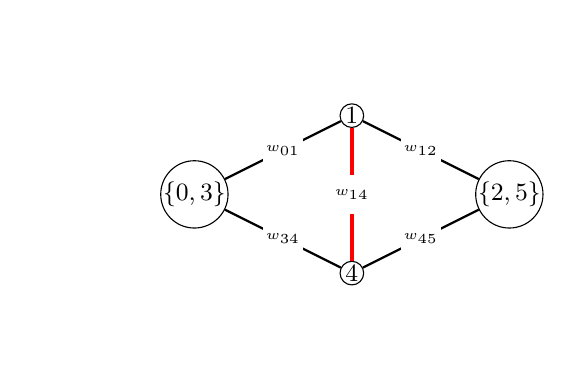
\begin{tikzpicture}
    \draw (0,-1)node (dummyLow){} ;
    \draw (0, 3)node (dummyLow){} ;
    \draw (2,1) node[nS] (n03) {$\{0,3\}$}; 
    \draw (4,2) node[nS] (n1) {$1$};
    \draw (6,1) node[nS] (n25) {$\{2,5\}$};
    \draw (4,0) node[nS] (n4) {$4$};
    \path
        (n03) edge[eS] node[eNS]{$w_{01}$} (n1) 
        (n1) edge[eS] node[eNS]{$w_{12}$} (n25) 
        (n03) edge[eS] node[eNS]{$w_{34}$} (n4) 
        (n4) edge[eS] node[eNS]{$w_{45}$} (n25)
        (n1) edge[eC] node[eNS]{$w_{14}$} (n4)
    ;
    \end{tikzpicture}
    \begin{tikzpicture}
    \draw (0,-1)node (dummyLow){} ;
    \draw (0, 3)node (dummyLow){} ;
    \draw (2,1) node[nS] (n03) {$\{0,3\}$}; 
    \draw (4,1) node[nS] (n14) {$\{1,4\}$};
    \draw (6,1) node[nS] (n25) {$\{2,5\}$};
    \path
        %(n03) edge[eS] node[eNS]{$w_{01}$} (n1) 
        (n14) edge[eNC] node[eNS]{$w_{12}+$\\$w_{45}$} (n25) 
        (n03) edge[eS] node[eNS]{$w_{01}+$\\$w_{34}$} (n14) 
    ;
    \end{tikzpicture}
}
\caption{
    To use hierarchical clustering as an approximator for
    the multicut objective we contract the edge with the highest weight
    in each step (to be contracted edge is shown in red). 
    Whenever multiple edges are merged into a single edge,
    we use the sum of the weight as a new weight, since
    we have to pay for all edges which are cut in the uncontracted 
    graph.
    We stop when the highest edge weight is smaller
    or equal to zero (edge shown in green).
}\label{fig:hc_alg}
\end{figure}
\end{center}





Outside computer vision greedy methods has been suggested for correlation clustering problems, see \cite{Elsner-2009} for an overview.
A common greedy approach~\cite{Soon-2001,Ng-2002,Elsner-2008} is to randomly permute the nodes and than assign 
iteratively each node to an existing cluster or create a new cluster if costs cannot be decreased by assigning to a cluster.
%Common assigning strategies are:
%\emph{BEST}; assign to cluster which is linked by the most positive edge~\cite{Ng-2002},
%\emph{FIRST}; Assign to the cluster which is first linked by a positive edge~\cite{Soon-2001}, and
%\emph{VOTE}; Assign to cluster that minimizes objective function~\cite{Elsner-2008}.
%
The PIVOT Algorithm~\cite{Ailon-2008} iterate over all nodes in random order.
If the node is not assigned it construct a cluster containing the node and all its 
unassigned positively linked neighbors.  
%
%Typically these algorithms started for many random permutations, 
%and pick the clustering with best objective value.

A widely use post-processing method is  Best One Element Move (BOEM)~\cite{Gionis-2007}.
Start with an initial clustering one node is removed from a cluster and reassigned to an existing or new cluster such that the costs are minimized.
BEOM stops if no move can decrease the costs.

% \subsection{Karger-Stein Algorithms}
% Use randomized procedure to reduce the number of nodes / edges to a reasonable 
% number.
% On the smaller graph, more expensive solvers are used.


%%!TEX root = ../egpaper_for_review.tex

\tikzstyle{nS}=[circle,minimum size = 0.3cm,inner sep = 0pt,draw, font=\small,align=left]
\tikzstyle{eS}=[thick,minimum size = 0.5cm,inner sep = 0pt,draw, font=\small,align=left]
\tikzstyle{eC}=[very thick,minimum size = 0.5cm,inner sep = 0pt,draw=red, font=\small,align=left]
\tikzstyle{eNC}=[very thick,minimum size = 0.5cm,inner sep = 0pt,draw=green, font=\small,align=left]
\tikzstyle{eNS}=[fill=white,minimum size = 0.5cm,inner sep = 0pt, font=\tiny,align=left]

\begin{center}
\begin{figure}
\resizebox{!}{0.30\linewidth}{%
    \begin{tikzpicture}
    \draw (0,-1)node (dummyLow){} ;
    \draw (0, 3)node (dummyLow){} ;
    \draw (2,2) node[nS] (n0) {$0$}; 
    \draw (4,2) node[nS] (n1) {$1$};
    \draw (6,2) node[nS] (n2) {$2$};
    \draw (2,0) node[nS] (n3) {$3$}; 
    \draw (4,0) node[nS] (n4) {$4$};
    \draw (6,0) node[nS] (n5) {$5$};


    \path
        (n0) edge[eS] node[eNS]{$w_{01}$} (n1) 
        (n1) edge[eS] node[eNS]{$w_{12}$} (n2) 
        (n3) edge[eS] node[eNS]{$w_{34}$} (n4) 
        (n4) edge[eS] node[eNS]{$w_{45}$} (n5)
        (n0) edge[eC] node[eNS]{$w_{03}$} (n3)
        (n1) edge[eS] node[eNS]{$w_{14}$} (n4)
        (n2) edge[eS] node[eNS]{$w_{25}$} (n5)
    ;
    \end{tikzpicture}
    \begin{tikzpicture}
    \draw (0,-1)node (dummyLow){} ;
    \draw (0, 3)node (dummyLow){} ;
    \draw (2,1) node[nS] (n03) {$\{0,3\}$}; 
    \draw (4,2) node[nS] (n1) {$1$};
    \draw (6,2) node[nS] (n2) {$2$};
    \draw (4,0) node[nS] (n4) {$4$};
    \draw (6,0) node[nS] (n5) {$5$};


    \path
        (n03) edge[eS] node[eNS]{$w_{01}$} (n1) 
        (n1) edge[eS] node[eNS]{$w_{12}$} (n2) 
        (n03) edge[eS] node[eNS]{$w_{34}$} (n4) 
        (n4) edge[eS] node[eNS]{$w_{45}$} (n5)
        (n1) edge[eS] node[eNS]{$w_{14}$} (n4)
        (n2) edge[eC] node[eNS]{$w_{25}$} (n5)
    ;
    \end{tikzpicture}
}


\resizebox{!}{0.30\linewidth}{%
    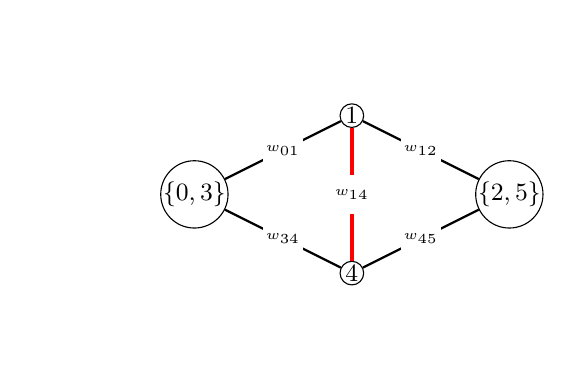
\begin{tikzpicture}
    \draw (0,-1)node (dummyLow){} ;
    \draw (0, 3)node (dummyLow){} ;
    \draw (2,1) node[nS] (n03) {$\{0,3\}$}; 
    \draw (4,2) node[nS] (n1) {$1$};
    \draw (6,1) node[nS] (n25) {$\{2,5\}$};
    \draw (4,0) node[nS] (n4) {$4$};
    \path
        (n03) edge[eS] node[eNS]{$w_{01}$} (n1) 
        (n1) edge[eS] node[eNS]{$w_{12}$} (n25) 
        (n03) edge[eS] node[eNS]{$w_{34}$} (n4) 
        (n4) edge[eS] node[eNS]{$w_{45}$} (n25)
        (n1) edge[eC] node[eNS]{$w_{14}$} (n4)
    ;
    \end{tikzpicture}
    \begin{tikzpicture}
    \draw (0,-1)node (dummyLow){} ;
    \draw (0, 3)node (dummyLow){} ;
    \draw (2,1) node[nS] (n03) {$\{0,3\}$}; 
    \draw (4,1) node[nS] (n14) {$\{1,4\}$};
    \draw (6,1) node[nS] (n25) {$\{2,5\}$};
    \path
        %(n03) edge[eS] node[eNS]{$w_{01}$} (n1) 
        (n14) edge[eNC] node[eNS]{$w_{12}+$\\$w_{45}$} (n25) 
        (n03) edge[eS] node[eNS]{$w_{01}+$\\$w_{34}$} (n14) 
    ;
    \end{tikzpicture}
}
\caption{
    To use hierarchical clustering as an approximator for
    the multicut objective we contract the edge with the highest weight
    in each step (to be contracted edge is shown in red). 
    Whenever multiple edges are merged into a single edge,
    we use the sum of the weight as a new weight, since
    we have to pay for all edges which are cut in the uncontracted 
    graph.
    We stop when the highest edge weight is smaller
    or equal to zero (edge shown in green).
}\label{fig:hc_alg}
\end{figure}
\end{center}




